%%%%%%%%%%%%%%%%%%%%%%%%%%%%% Define Article %%%%%%%%%%%%%%%%%%%%%%%%%%%%%%%%%%
\documentclass[addpoints]{exam}
%%%%%%%%%%%%%%%%%%%%%%%%%%%%%%%%%%%%%%%%%%%%%%%%%%%%%%%%%%%%%%%%%%%%%%%%%%%%%%%

%%%%%%%%%%%%%%%%%%%%%%%%%%%%% Using Packages %%%%%%%%%%%%%%%%%%%%%%%%%%%%%%%%%%
\usepackage{amsmath}
\usepackage{amssymb}
\usepackage{geometry}
\usepackage{venndiagram}
\usepackage{graphicx}
\usepackage{float}
\usepackage[breaklinks]{hyperref}
\usepackage{listings}
\usepackage{pdfpages}
\usepackage{comment}
\usepackage{empheq}
\usepackage{mdframed}
\usepackage{booktabs}
\usepackage{lipsum}
\usepackage{color}
\usepackage{wrapfig}
\usepackage{bookmark}
\usepackage{titlesec}
\usepackage{hyperref}
\usepackage{parskip}
\usepackage{empheq}
\usepackage{verbatim}
\usepackage{subfig}
%%%%%%%%%%%%%%%%%%%%%%%%%%%%%%%%%%%%%%%%%%%%%%%%%%%%%%%%%%%%%%%%%%%%%%%%%%%%%%%

% Other Settings

%%%%%%%%%%%%%%%%%%%%%%%%%% Page Setting %%%%%%%%%%%%%%%%%%%%%%%%%%%%%%%%%%%%%%%
% \renewcommand{\solution}{\noindent}
\geometry{a4paper}
\printanswers
\qformat{}

%%%%%%%%%%%%%%%%%%%%%%%%%% Define some useful colors %%%%%%%%%%%%%%%%%%%%%%%%%%
\definecolor{ocre}{RGB}{243,102,25}
\definecolor{mygray}{RGB}{243,243,244}
\definecolor{deepGreen}{RGB}{26,111,0}
\definecolor{shallowGreen}{RGB}{235,255,255}
\definecolor{deepBlue}{RGB}{61,124,222}
\definecolor{shallowBlue}{RGB}{235,249,255}
%%%%%%%%%%%%%%%%%%%%%%%%%%%%%%%%%%%%%%%%%%%%%%%%%%%%%%%%%%%%%%%%%%%%%%%%%%%%%%%

%%%%%%%%%%%%%%%%%%%%%%%%%% Define an orangebox command %%%%%%%%%%%%%%%%%%%%%%%%
\newcommand\orangebox[1]{\fcolorbox{ocre}{mygray}{\hspace{1em}#1\hspace{1em}}}
%%%%%%%%%%%%%%%%%%%%%%%%%%%%%%%%%%%%%%%%%%%%%%%%%%%%%%%%%%%%%%%%%%%%%%%%%%%%%%%

%%%%%%%%%%%%%%%%%%%%%%%%%%%%%%% Title & Author %%%%%%%%%%%%%%%%%%%%%%%%%%%%%%%%
\title{Operating Systems - CS/CE 232L/324L\\ Lab 14: Signals in Depth}
\author{Ali Muhammad Asad - aa07190}
\date{} %Leave uncommented if u want automatic date which is done through maketitle, else u can uncomment this and type anything else u want over here - not necessary to enter a date over here
%%%%%%%%%%%%%%%%%%%%%%%%%%%%%%%%%%%%%%%%%%%%%%%%%%%%%%%%%%%%%%%%%%%%%%%%%%%%%%%

\begin{document}
\maketitle

% \begin{center}
%     \gradetable[h]
% \end{center}

\vspace*{5mm}
\begin{questions}
    \question
    \textbf{Example 1:} \texttt{\textcolor{red}{kill -9 <pid>}}
    \begin{figure}[htbp]
        \centering
        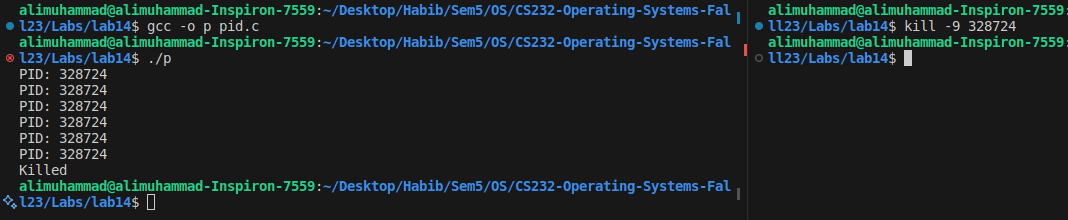
\includegraphics[width=0.925\textwidth]{eg1.png}
        \caption*{Example 1: Using \texttt{kill -9} to kill a process}
    \end{figure}
    
    \question
    \textbf{Example 2:} \texttt{\textcolor{red}{kill -s USR1 <pid>}}
    \begin{figure}[htbp]
        \centering
        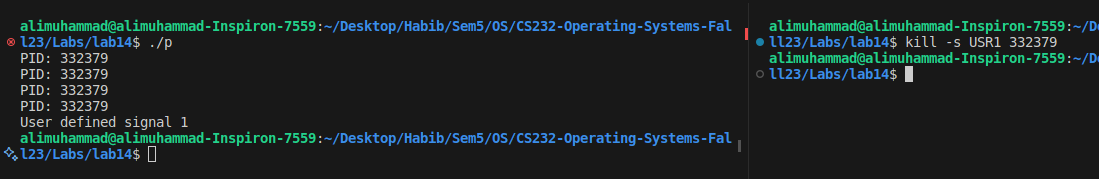
\includegraphics[width=0.925\textwidth]{eg2.png}
        \caption*{Example 2: Using \texttt{kill -s USR1} to send a signal to a process}
    \end{figure}
    
    \pagebreak
    \question
    \textbf{Example 4:} \texttt{\textcolor{red}{if (kill(3423, SIGUR1) == -1)}}
    \begin{figure}[htbp]
        \centering
        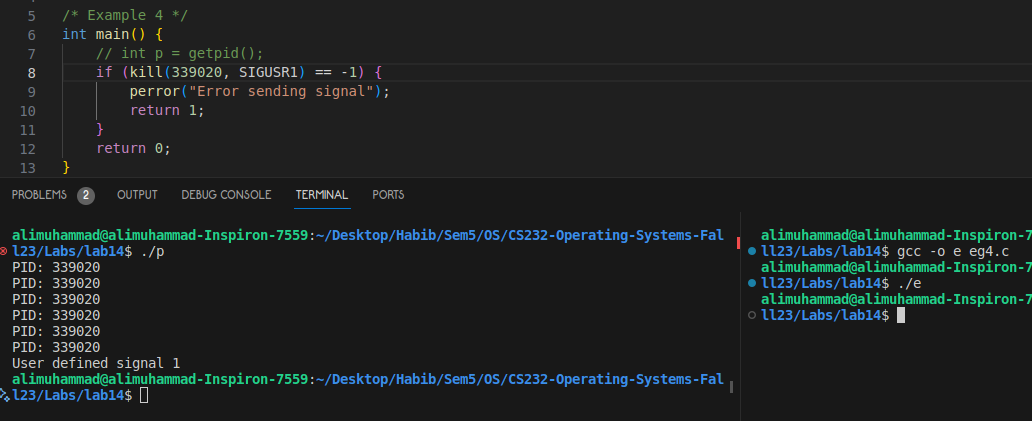
\includegraphics[width=0.925\textwidth]{eg4.png}
        \caption*{Example 4: Using \texttt{kill()} to send a signal to a process}
    \end{figure}
    
    \question
    \textbf{Example 5:} Child murders its parent
    \begin{figure}[H]
        \centering
        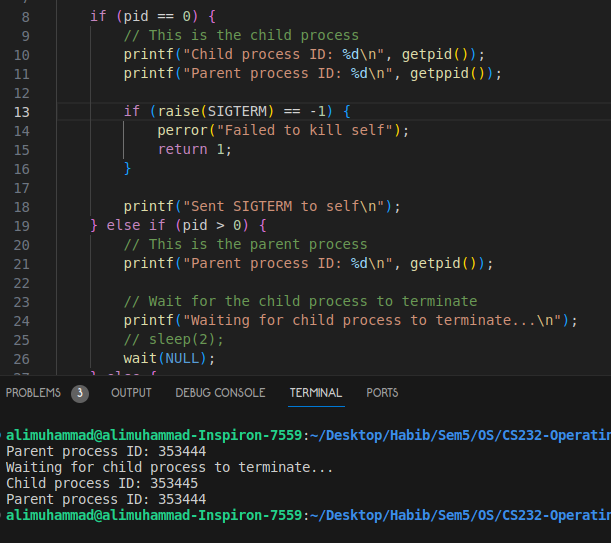
\includegraphics[width=0.75\textwidth]{eg5.png}
        \caption*{Example 5: Child murders its parent}
    \end{figure}
    
    \question
    \textbf{Example 6:} Process commits suicide; sends signal to kill itself
    \begin{figure}[H]
        \centering
        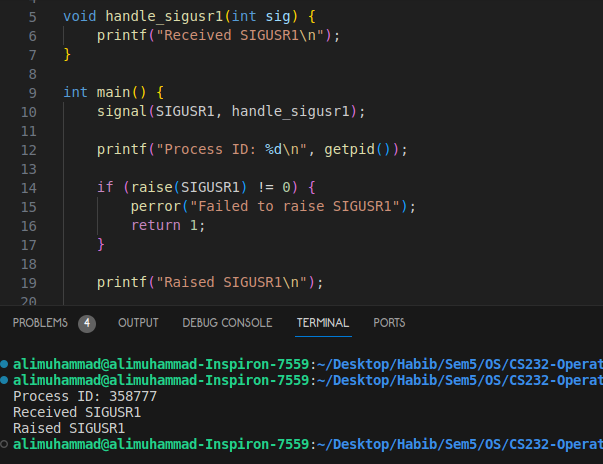
\includegraphics[width=0.75\textwidth]{eg6.png}
        \caption*{Example 6: Oh no process suicided - reason? This lab}
    \end{figure}
    
    \question
    \textbf{Example 7:} \texttt{\textcolor{red}{simplealarm.c}}
    \begin{figure}[H]
        \centering
        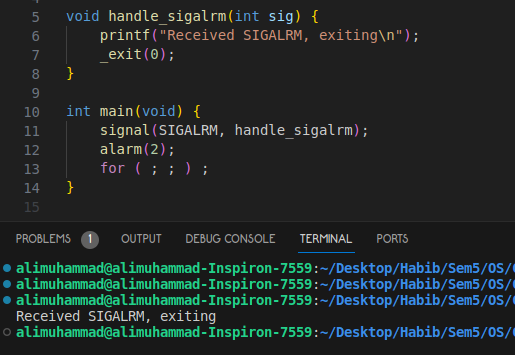
\includegraphics[width=0.75\textwidth]{eg7.png}
        \caption*{Example 7: Alarm}
    \end{figure}
    
    \question
    \textbf{Example 8:} \texttt{\textcolor{red}{SIGINT}} and \texttt{\textcolor{red}{SIGQUIT}}
    \begin{figure}[H]
        \centering
        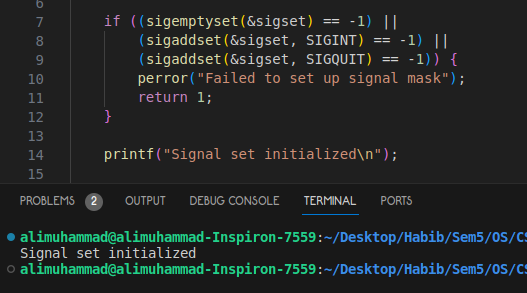
\includegraphics[width=0.75\textwidth]{eg8.png}
        \caption*{Example 8}
    \end{figure}
    
    \question
    \textbf{Example 9:} \texttt{\textcolor{red}{sigset\_t newsigset}} blocking signals
    \begin{figure}[H]
        \centering
        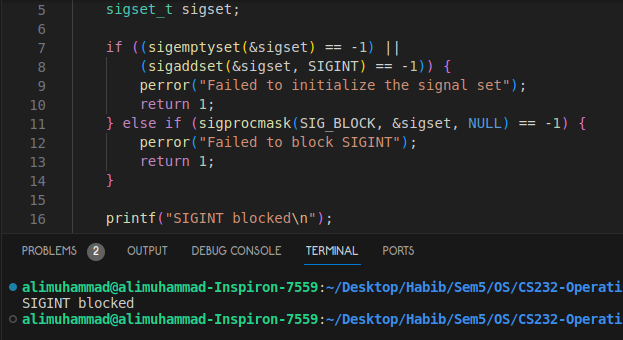
\includegraphics[width=0.75\textwidth]{eg9.png}
        \caption*{Example 9}
    \end{figure}
    
    \pagebreak
    \question
    \textbf{Question 1:} Is it possible that after a call to \textcolor{red}{`makepair'} \textcolor{red}{`pipe1'} exists but \textcolor{red}{`pipe2'} does not?
    \begin{solution}
        Yes its possible. The function attempts to create two named pipes (FIFOs) using mkfifo for pipe1 and pipe2. If pipe1 gets created successfully but pipe2 fails (due to lack of permissions or space etc, that could set errno to something other than EEXIST), the function will not remove pipe1 before it returns. In this scenario, pipe1 would exist, but pipe2 would not.
    \end{solution}

    \question
    \textbf{Question 2:} Does a \textcolor{red}{`makepair'} return value of 0 guarantee that FIFOs corresponding to \textcolor{red}{`pipe1'} and \textcolor{red}{`pipe2'} are available on return?
    \begin{solution}
        A return value of 0 from makepair does indeed guarantee that both FIFOs corresponding to pipe1 and pipe2 have been successfully created and are available for use. The function only returns 0 if both mkfifo calls succeed (ignoring the case where either FIFO already exists, as indicated by errno == EEXIST). If any step of the FIFO creation process or the signal mask restoration with sigprocmask fails, the function cleans up by unlinking any FIFOs that might have been created during this call and returns -1.
    \end{solution}
    
    
    \question
    \textbf{Example 10:} \texttt{\textcolor{red}{mysighand}}
    \begin{figure}[H]
        \centering
        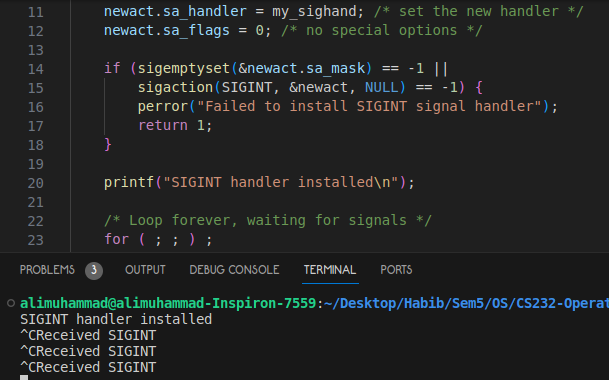
\includegraphics[width=0.75\textwidth]{eg10.png}
        \caption*{Example 10}
    \end{figure}
    \pagebreak
    \question
    \textbf{Example 11:} \texttt{\textcolor{red}{struct sigaction act}}
    \begin{figure}[H]
        \centering
        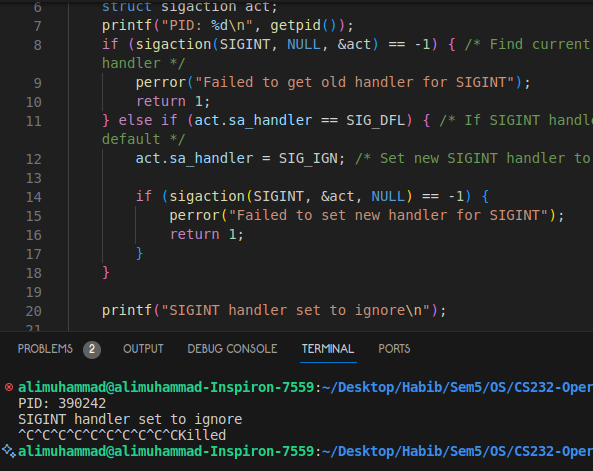
\includegraphics[width=0.65\textwidth]{eg11.png}
        \caption*{Example 11}
    \end{figure}

    \question
    \textbf{Example 12:} \texttt{\textcolor{red}{catchctrlc(int signo)}}
    \begin{figure}[H]
        \centering
        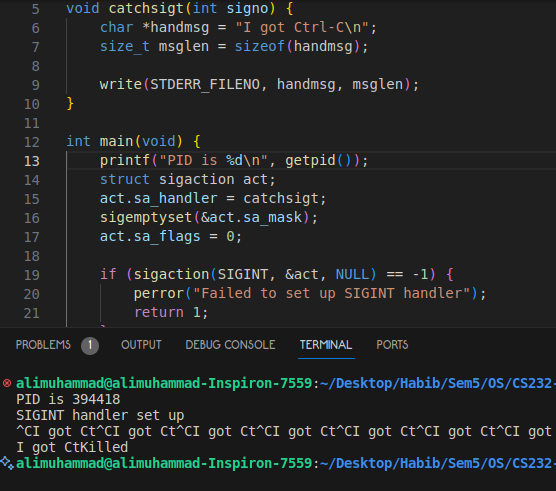
\includegraphics[width=0.65\textwidth]{eg12.png}
        \caption*{Example 12}
    \end{figure}

    \question
    \textbf{Question 3:} Why didn't \textcolor{blue}{Example 12} use \textcolor{red}{fprintf} or \textcolor{red}{strlen} in the signal handler?
    \begin{solution}
        In the context of signal handlers, it is important to use functions that are async-signal-safe. When a signal handler is invoked, it interrupts the normal flow of the program execution. If such functions are called again from a signal handler, it could lead to data corruption or undefined behaviour. \textcolor{red}{fprintf} and \textcolor{red}{strlen} are not async-signal-safe functions, and could interact with buffered I/O or cause unpredictable results if a signal occurs. \textcolor{red}{write} is used instead since it is async-signal-safe that directly interacts with file desriptors without buffering.
    \end{solution}

    \question
    \textbf{Example 13:} \texttt{\textcolor{red}{testignored}}
    \begin{figure}[H]
        \centering
        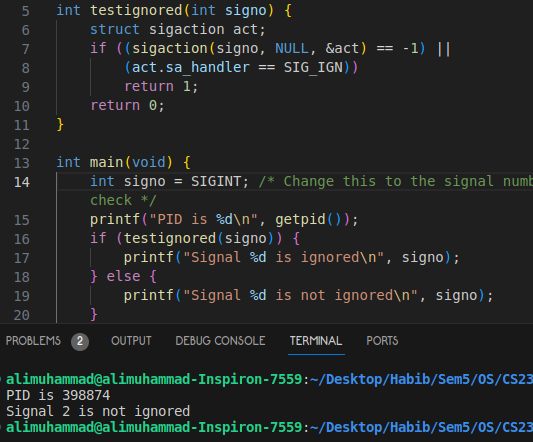
\includegraphics[width=0.65\textwidth]{eg13.png}
        \caption*{Example 13}
    \end{figure}
    
\end{questions}
\end{document}